\documentclass[11pt, oneside]{article}   	% use "amsart" instead of "article" for AMSLaTeX format
\usepackage{geometry}                		% See geometry.pdf to learn the layout options. There are lots.
\geometry{letterpaper}                   		% ... or a4paper or a5paper or ... 
%\geometry{landscape}                		% Activate for for rotated page geometry
%\usepackage[parfill]{parskip}    		% Activate to begin paragraphs with an empty line rather than an indent
\usepackage{graphicx}				% Use pdf, png, jpg, or eps� with pdflatex; use eps in DVI mode
								% TeX will automatically convert eps --> pdf in pdflatex		
\usepackage{amssymb}
\usepackage{amsmath}
\usepackage{parskip}
\usepackage{color}

\title{Elastic collisions}
%\author{The Author}
%\section{}
%\subsection*{}
\date{}							% Activate to display a given date or no date

\graphicspath{{/Users/telliott_admin/Dropbox/Tex/png/}}
% \begin{center} 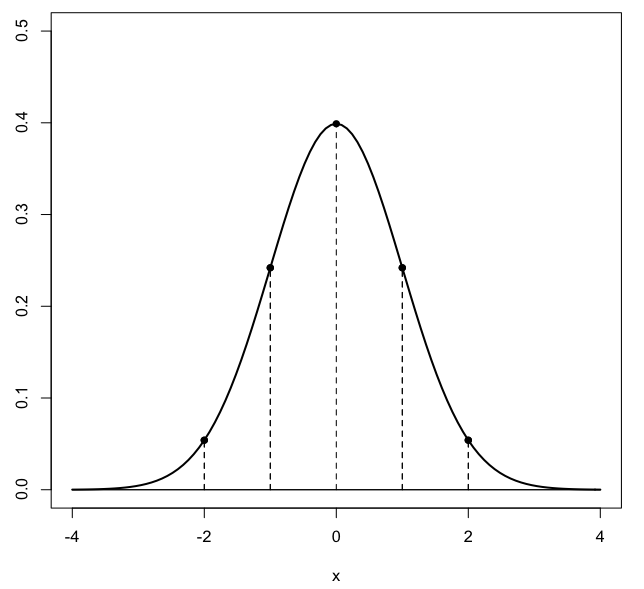
\includegraphics [scale=0.4] {gauss3.png} \end{center}
\begin{document}
\maketitle
\Large
For an elastic collision, energy is conserved.  Call $v$ the velocity before collision and $w$ the velocity after
\[ \frac{1}{2}m_1 v_1^2 + \frac{1}{2}m_2 v_2^2 = \frac{1}{2}m_1 w_1^2 + \frac{1}{2}m_2 w_2^2 \]
Rearrange (and multiply by $2$):
\[ m_1 v_1^2 - m_1 w_1^2 = m_2 w_2^2 - m_2 v_2^2 \]
Factor
\[ m_1(v_1 + w_1)(v_1 - w_1) = m_2 (w_2 + v_2)(w_2 - v_2) \]
Conservation of momentum gives
\[ m_1 v_1 + m_2 v_2 = m_1 w_1 + m_2 w_2 \]
Rearrange the momentum equation and factor out the masses
\[ m_1(v_1-w_1) = m_2(w_2-v_2) \]
Divide to obtain
\[ v_1 + w_1 = v_2 +  w_2 \]
\subsection*{solve this linear system for $w_1$ by eliminating $w_2$}
Isolate $w_2$ 
\[ w_2 = v_1 + w_1 - v_2 \]
multiply everything by $m_2$
\[ m_2 w_2 = m_2 v_1 + m_2 w_1 - m_2 v_2 \]
Go back to the momentum equation, isolate $m_2 w_2$
\[ m_2 w_2 = m_1 v_1 + m_2 v_2 - m_1 w_1  \]
Equate:
\[ m_2 v_1 + m_2 w_1 - m_2 v_2 = m_1 v_1 + m_2 v_2 - m_1 w_1 \]
Gather terms containing $w_1$
\[  m_2 w_1 + m_1 w_1 = m_1 v_1 + m_2 v_2 - m_2 v_1 + m_2 v_2  \]
\[ (m_1+m_2) w_1 = (m_1 -m_2) v_1 + 2 m_2 v_2 \]
Divide by $M = m_1 + m_2$ to reach
\[ w_1 = \frac{m_1 - m_2}{M}v_1 + \frac{2 m_2}{M} v_2 \]
We have the final velocity for $m_1$ in terms of the masses and the velocities of the objects before the collision.

Write the result with $v'$ rather than $w$ for those who like it that way:
\[ v_1' = \frac{m_1 - m_2}{M}v_1 + \frac{2 m_2}{M} v_2 \]

The equation for $v_2'$ is obtained by symmetry (switch $1$ for $2$ as needed):
\[ v_2' = \frac{m_2 - m_1}{M}v_2 + \frac{2 m_1}{M} v_1 \]
Note that in the case where $m_1 = m_2$
\[ v_1' = v_2 \]
and similarly, $v_2' = v_1$.

\subsection*{Atwood machine}
I ran into very similar equations in what seems to be a different context (in Fitzpatrick, Chapter 4).  There is a device called an "Atwood machine".
\begin{center} 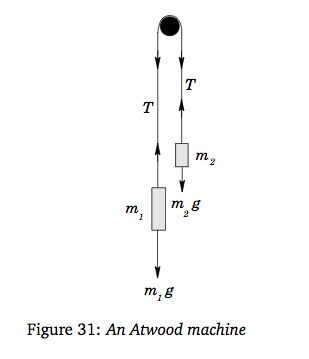
\includegraphics [scale=0.75] {Atwood.png} \end{center}
(massless, friction-less pulley, etc.)  If mass $m_1$ is bigger, then it will move downward.  

\emph{As a sign convention, assume that a is positive downward for $m_1$ and positive upward for $m_2$}.  Then, the forces on $m_1$ and $m_2$ are
\[ m_1a = m_1g - T  \]
\[ m_2a = T - m_2g  \]
By addition
\[ m_1a + m_2a = m_1g - m_2g  \]
\[ a = \frac{m_1 - m_2}{m_1 + m_2} g  \]
Alternatively, by solving for $a$ and equating we obtain
\[ g - \frac{T}{m_1} = \frac{T}{m2} - g \]
\[ 2g = T (\frac{1}{m_1} + \frac{1}{m_2})\]
\[ 2g = T (\frac{m_1 + m_2}{m_1 m_2})\]
\[ T = g\frac{2 m_1 m_2}{m_1 + m_2} \]
Not sure if there is a connection.

\end{document}  